\chapter{Additional Runtime Support}
In this chapter we will address some remaining issues of the replication system.
%please expand this part

\section{System Call Synchronization}
% put syscall hooks here??
During the execution of an application, for most of the system calls, given the same external input, the application on both primary and secondary can produce the same result, however there are still some system calls that are intrinsically non-deterministic, which will lead to divergence of the execution on all the replicas. As a result we have to synchronize the output of them to ensure the consistent final output of the applications on both sides.

\paragraph{Disabling vDSO}

vDSO(virtual dynamic shared object) is a mechanism that allows a system call to be done in user space, instead of having context switch to the kernel space. This is done by having a shared memory section between the user space and the kernel. When the system call is initiated, the corresponding function in the vDSO library is called instead of trapping into the kernel, then the library will fetch the result from this shared memory area and return. This boosts the performance for some "read only" system calls (like gettimeofday/time). However, in our case, if the system call doesn't go into the kernel space, we cannot track and synchronize them. Also, in order to synchronize the system call data we have to get into the kernel space anyway to send inter-kernel messages. So vDSO in our context becomes a burden to the implementation. As a result in our system we have to disable vDSO.

In our implementation we only synchronize those system calls that are strongly related to network I/O: gettimeofday/time, poll, epoll\_wait. We didn't implement select because it is relatively out-dated, modern network applications hardly use it, as a result it doesn't worth to put any effort into it. In the following subsections we will describe each synchronized system call in detail. 

\subsection{gettimeofday/time}

gettimeofday and time are used for getting the current timestamp. Since the primary and secondary can not always have the same execution progress, the timing of calling gettimeofday/time might be different. For those applications that the output is time related, those system calls will cause output divergence. For gettimeofday/time, the primary simply copies the result to the secondary, when secondary executes the corresponding gettimeofday/time, it directly uses the output from the primary and bypasses it's original path.

\subsection{poll}

poll is used for waiting on a set of file descriptors for I/O. A programmer can register a set of file descriptors to poll along with the type of events that is related to those file descriptors. poll takes an array of pollfd struct as shown in Figure~\ref{f:pollfd}. When it is called, it waits until one or more registered file descriptors become ready with registered events. When it returns, it fills the array with those file descriptors that are ready and returns the number of ready file descriptors. The user space application iterates the array and reacts to each file descriptor according to the events and revents field.

\begin{figure}
\begin{lstlisting}[numbers=left, frame=single, basicstyle=\small, breaklines]{poll}
int poll(struct pollfd *fds, nfds_t nfds, int timeout);

struct pollfd {
    int   fd;         /* file descriptor */
    short events;     /* requested events */
    short revents;    /* returned events */
};
\end{lstlisting}
\caption{poll prototype and pollfd data structure}
\label{f:pollfd}
\end{figure}

poll notification mechanism relies on the Linux VFS subsystem. However, as described in previous chapter, on the secondary kernel the replicated TCP/IP stack will bypass the original execution path for accept/read/write on sockets, in other words, the VFS subsystem is partially bypassed. As a result, poll will not be woken up properly on the secondary even when the event already arrives, which leads to a different output other than the primary.

The solution is similar to time/gettimeofday, we simply send the output of poll to the secondary. As shown in Figure~\ref{f:pollfd}, the output of poll is the fds array and the return value. Upon receives the information, the secondary uses this as the output of itself and bypasses its original execution path.

\subsection{epoll\_wait}
Similar to poll, epoll\_wait is also used for waiting on a set of file descriptors for I/O. It waits on a set of registered file descriptors and outputs the ready ones to an epoll\_event array. Due to the implementation of our replicated network stack, epoll mechanism has the same problem as poll. Figure~\ref{f:epoll} shows the prototype of epoll\_wait and epoll\_event structure. Compare to the relatively simpe pollfd structure, epoll\_event contains a data field which can be an arbitrary data structure. It is OK to just copy the data field to the other side if it only contains integers. However if this field is a pointer, due to the non-determinism of memory address on both side, simply passing the pointer to the other side may lead to an illegal memory access. As a result, on the secondary, along the output path of epoll\_wait, we need to find the corresponding data structure in its own address space.

On the primary kernel, once the epoll\_wait is ready to return, it will send a message which contains the current epfd, all the ready file descriptors and the value of events field of every file descriptor. Upon the secondary receives the message, it will search the RB tree associated to the given epfd, find the previous registered epoll\_event of the ready file descriptors, and overrides the events field with the information from the primary. At the end, return to the user space with the array of epoll\_event and bypass the original epoll\_wait execution.

\begin{figure}
\begin{lstlisting}[numbers=left, frame=single, basicstyle=\small, breaklines]{epoll}
int epoll_wait(int epfd, struct epoll_event *events,
                      int maxevents, int timeout);

typedef union epoll_data {
    void    *ptr;
    int      fd;
    uint32_t u32;
    uint64_t u64;
} epoll_data_t;

struct epoll_event {
    uint32_t     events;    /* Epoll events */
    epoll_data_t data;      /* User data variable */
};

\end{lstlisting}
\caption{epoll\_wait prototype and epoll\_event data structure}
\label{f:epoll}
\end{figure}

\section{Override Pthread Library}
In Chapter~\ref{chap:detexec} and Chapter~\ref{chap:schedrep} we described how to wrap the pthread primitives with \_\_det\_start and \_\_det\_end to ensure the same thread interleaving for the replicated application on the primary and the secondary. Manually instrument the code is tedious, one has to find every single pthread primitive in the code. Moreover, if an application uses an external library that uses pthread, it will be even more troublesome to recompile the needed external library. An intuitive solution is to modify the pthread library and wrap our \_\_det\_start and \_\_det\_end directly in the pthread code. However updating the glibc of a system can be very dangerous and might harm other applications that don't need to be replicated.

\paragraph{LD\_PRELOAD}
In Linux, the behaviour of the dynamic linker can be altered by setting LD\_PRELOAD environment variable. This can change the runtime linking process and make the linker to search for symbols in the path defined in LD\_PRELOAD. With this trick we are able to alter the behaviour of glibc without actually changing it. We implemented our LD\_PRELOAD library with instrumented pthread function in it, and the namespace launching script will automatically set LD\_PRELOAD to be the path of our library, so that only the application running in the namespace will be affected by our LD\_PRELOAD library. In the upcoming sections we will describe how we wrap pthread functions in our LD\_PRELOAD library.

\subsection{Override Lock Functions}

Figure~\ref{f:orverridelocks} shows the implementation of pthread\_mutex\_lock in our LD\_PRELOAD library. Line 9 loads the real pthread\_mutex\_lock function from the real pthread library, in Line 12 we simply call this function with \_\_det\_start and \_\_det\_end wrapped around. In our LD\_PRELOAD library, we wrapped all the pthread lock functions include pthread\_mutex\_lock, pthread\_mutex\_trylock, pthread\_rwlock\_rdlock, pthread\_rwlock\_tryrdlock, pthread\_rwlock\_wrlock, pthread\_rwlock\_trywrlock.

\begin{figure}
\begin{lstlisting}[numbers=left, frame=single, basicstyle=\small, breaklines]{locks}
int pthread_mutex_lock(pthread_mutex_t *mutex)
{
    int ret;
    static int (*pthread_mutex_lock_real)(pthread_mutex_t *mutex) = NULL;    
    if (!handle) {
        handle = dlopen(PTHREAD_PATH, RTLD_LAZY);
    }
    if (!pthread_mutex_lock_real)
        pthread_mutex_lock_real = dlsym(handle, "pthread_mutex_lock");

    syscall(__NR_det_start);
    ret = pthread_mutex_lock_real(mutex);
    syscall(__NR_det_end);

    return ret;
}
\end{lstlisting}
\caption{pthread\_mutex\_lock in the LD\_PRELOAD library}
\label{f:orverridelocks}
\end{figure}

\subsection{Override Condition Variable Functions}

Condition Variables are much more complicated than mutex locks. In the glibc implementation, it involves multiple internal lock and unlock operations. As a result simply wrapping pthread\_cond\_wait with \_\_det\_start and \_\_det\_end will not work, because of multiple non-deterministic execution points are inside the implementation. Figure~\ref{f:cond_wait} shows the brief flow of the pthread\_cond\_wait in glibc implementation. cond->lock is a lock inside the condition variable  data structure, it is used to provide mutual exclusion for the futex value for the condition variable. futex\_wait will wait until cond\->futex differs from futex\_val. When it wakes up, it will check again if this condition variable is contended, if so, go back to futex\_wait again. If not, re-acquire the mutex lock and return. Every single lock acquisition here is a non-deterministic point, which leads to passing different values to futex\_wait on primary and replica, which in turn leads to diverged wakeup timing of pthread\_cond\_wait.

In our LD\_PRELOAD library, we re-implemented pthread\_cond\_wait following the existing glibc\'s implementation, and wrapped every single lock acquisition with \_\_det\_start and \_\_det\_end, we also did the same wrapping for pthread\_cond\_signal. With this, we are able to make sure that the pthread\_cond\_wait can return at the same timing with the same condition variable on both primary and secondary.

\begin{figure}
\centering
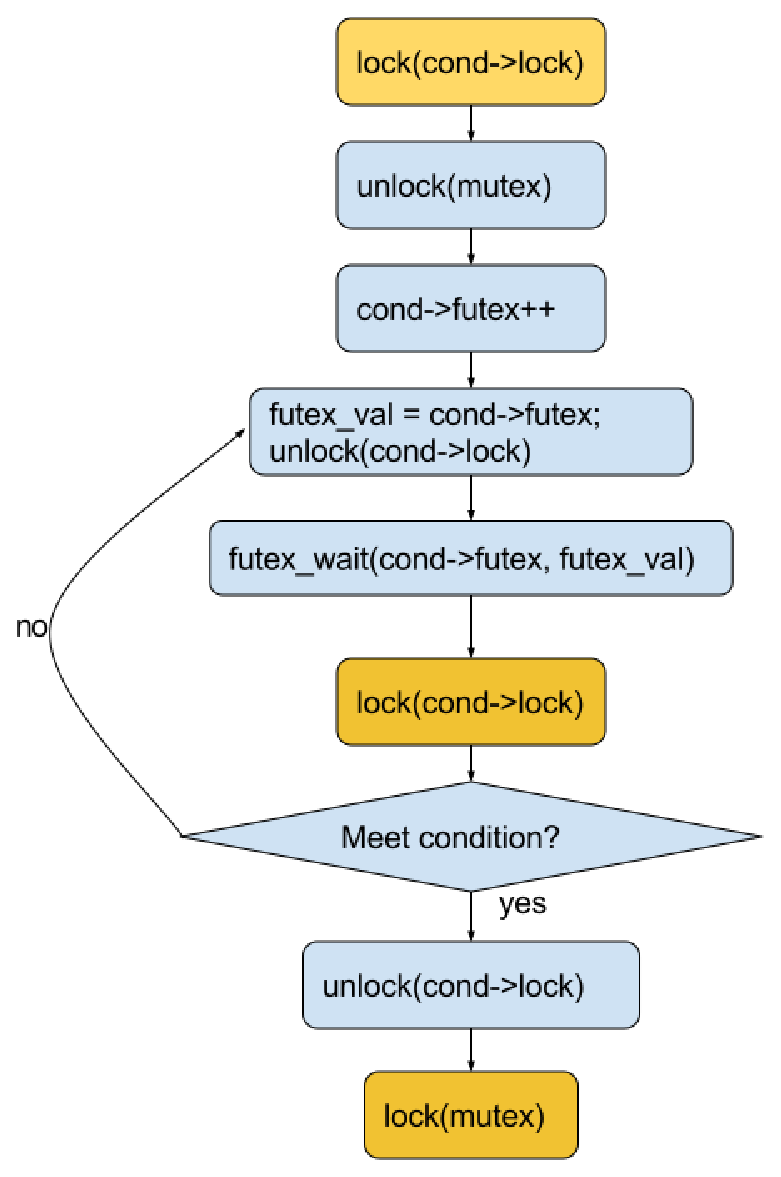
\includegraphics[width=0.4\columnwidth]{figures/cond_wait}
\caption{glibc pthread\_cond\_wait internal work flow}
\label{f:cond_wait}
\end{figure}

\section{STDIO and STDERR}

\section{Synchronization Exclusion}
% skip the next detstart